\begin{figure}
    \begin{center}
    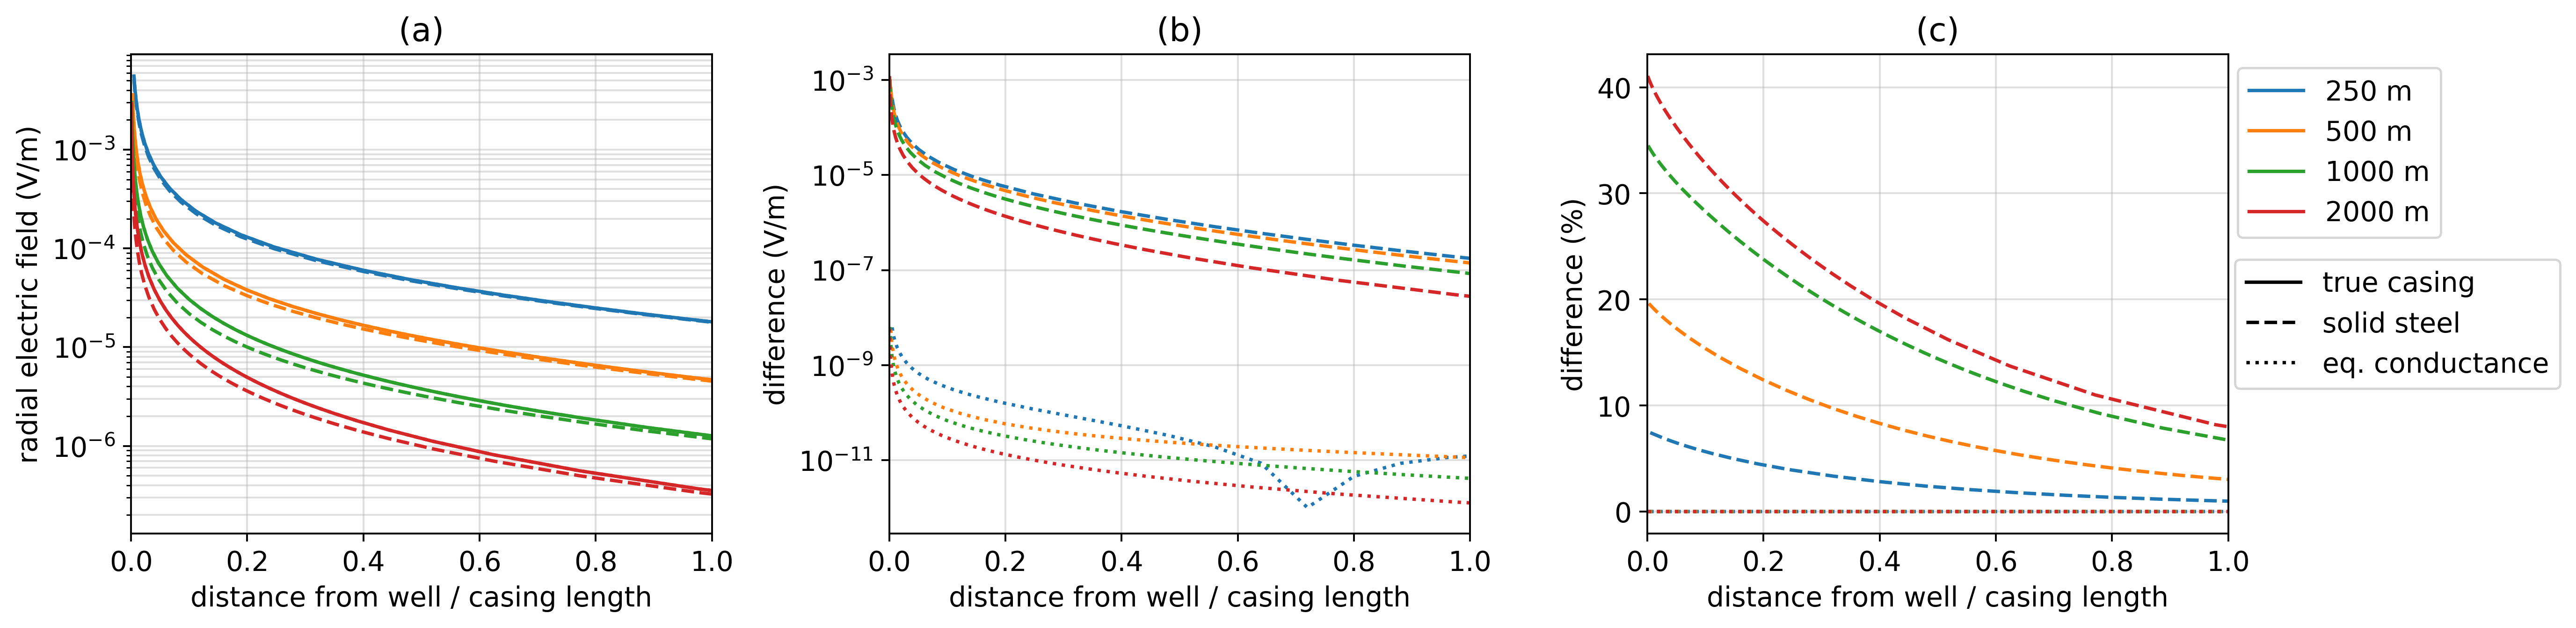
\includegraphics[width=\textwidth]{figures/approximating_wells_electric_fields.png}
    \end{center}
\caption{
    Radial electric field measured at the surface for a model of
    a hollow steel-cased well (solid lines), a solid cylinder with
    conductivity equal to that of the steel-cased well (dashed-lines),
    and a solid cylinder with a conductivity such that the product of the
    conductivity and the cross sectional area of the cylinder is equal to that
    of the hollow-pipe (dotted lines). Each of the line-colors corresponds to a
    different casing length, as indicated in the legend.
    In (a), we show the total radial electric field,
    (b) shows the difference in electric field from that due to the true, hollow-cased well,
    and (c) shows that difference as a percentage
    of the true electric fields.
    The x-axis on all plots is distance from the well normalized by the length of the casing.
}
\label{fig:approximating_wells_electric_fields}
\end{figure}
